\documentclass[UTF8]{ctexbeamer}

\usetheme{Pittsburgh}
\usefonttheme[onlymath]{serif}

\usepackage{subfig}
\usepackage{multirow}
\usepackage{xcolor,colortbl}
\usepackage{listings}
\usepackage{amsmath}

% Solarized colors
\definecolor{sbase03}{HTML}{002B36}
\definecolor{sbase02}{HTML}{073642}
\definecolor{sbase01}{HTML}{586E75}
\definecolor{sbase00}{HTML}{657B83}
\definecolor{sbase0}{HTML}{839496}
\definecolor{sbase1}{HTML}{93A1A1}
\definecolor{sbase2}{HTML}{EEE8D5}
\definecolor{sbase3}{HTML}{FDF6E3}
\definecolor{syellow}{HTML}{B58900}
\definecolor{sorange}{HTML}{CB4B16}
\definecolor{sred}{HTML}{DC322F}
\definecolor{smagenta}{HTML}{D33682}
\definecolor{sviolet}{HTML}{6C71C4}
\definecolor{sblue}{HTML}{268BD2}
\definecolor{scyan}{HTML}{2AA198}
\definecolor{sgreen}{HTML}{859900}

\lstset{
    % How/what to match
    sensitive=true,
    % Border (above and below)
    frame=lines,
    % Extra margin on line (align with paragraph)
    xleftmargin=\parindent,
    % Put extra space under caption
    belowcaptionskip=1\baselineskip,
    % Colors
    backgroundcolor=\color{sbase3},
    basicstyle=\color{sbase00}\ttfamily,
    keywordstyle=\color{scyan},
    commentstyle=\color{sbase1},
    stringstyle=\color{sblue},
    numberstyle=\color{sviolet},
    identifierstyle=\color{sbase00},
    % Break long lines into multiple lines?
    breaklines=true,
    % Show a character for spaces?
    showstringspaces=false,
    tabsize=2
}


% Title
\title{第11章 微分方程建模}
\author{韩建伟}
\institute{
  信息学院\\
  \texttt{hanjianwei@zjgsu.edu.cn}
}
\date{2019/12/11}

\begin{document}

% Title page
\begin{frame}[plain]
  \titlepage{}
\end{frame}

\begin{frame}{差分方程}
  
  \begin{block}{人口增长问题}
    $P$代表时刻$t$的人数数量,假设人口随时间的变化率依赖于当前人口数$P$及其它一些因素,则:
    \[
    \Delta P = P(t+\Delta t) - P(t) = kP\Delta t
    \]
  \end{block}

  \begin{figure}
    \centering
    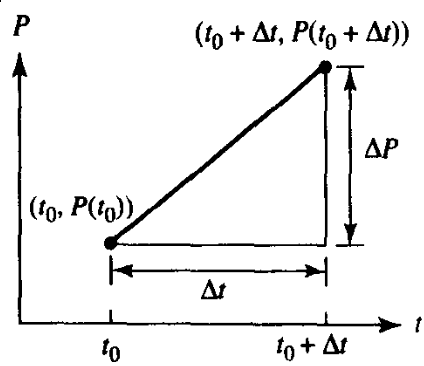
\includegraphics[width=0.4\textwidth]{diff.png}
  \end{figure}
  
\end{frame}

\begin{frame}{变化率}
  \begin{itemize}
  \item 平均变化率
    \[
    \frac{\Delta P}{\Delta t} = \frac{P(t+\Delta t) - P(t)}{\Delta t} = kP
    \]
  \item 瞬时变化率(让$\Delta t \rightarrow 0$):
    \[
    \lim_{\Delta t \rightarrow 0} \frac{\Delta P}{\Delta t} =\frac{d P}{d t} =kP
    \]
  \end{itemize}

  导数起着两种不同的作用:

  \begin{enumerate}
  \item 在连续问题中表示瞬时变化率
  \item 在离散问题中表示平均变化率
  \end{enumerate}

\end{frame}

\begin{frame}{导数作为变化率}
  \begin{figure}
    \centering
    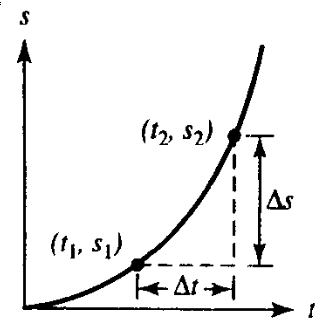
\includegraphics[width=0.2\textwidth]{dis.png}
    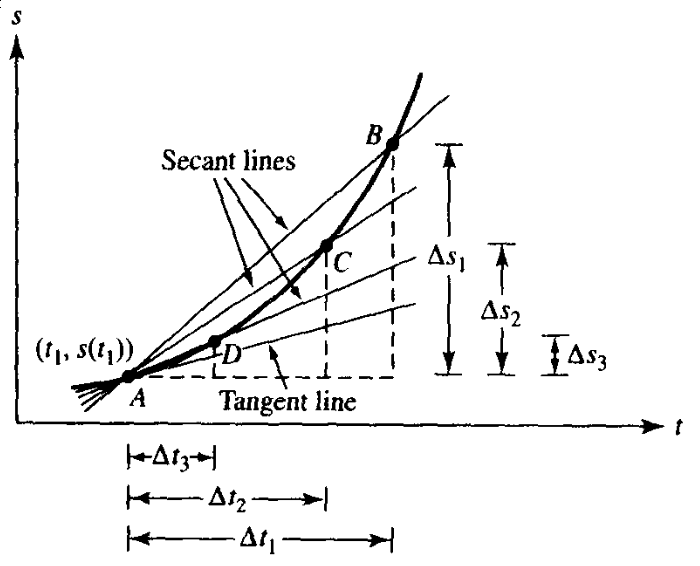
\includegraphics[width=0.4\textwidth]{slope.png}
  \end{figure}
  
  \[
  \begin{array}{c}
    \left.\frac{ds}{dt}\right|_{t=t_1}=\lim_{\Delta t \rightarrow 0}\frac{\Delta s}{\Delta t}
  \end{array}
  \]
\end{frame}

\begin{frame}{人口增长}
  \begin{block}{问题}
    $t = t_0$时刻人口数量为$P_0$,预测在未来某个$t=t_1$时刻的人口数量$P$。即,对于$t_0 \le t \le t_1$,找到人口关于时间的函数$P(t)$,满足$P(t_0)=P_0$.
  \end{block}
  \begin{itemize}
  \item 主要因素:出生率($b$)和死亡率$c$
  \item 次要因素(忽略):迁入迁出、生存空间的限制、可利用的水与食物、传染病
  \end{itemize}
  \[
  P(t+\Delta t) = P(t) + bP(t)\Delta t - cP(t)\Delta t
  \]
  \[
  \frac{\Delta P}{\Delta t} = bP - cP = kP
  \]
  \[
  \frac{dP}{dt} = kP, P(t_0)=P_0, t_0 \le t \le t_1
  \]
\end{frame}

\begin{frame}{马尔萨斯人口增长模型}
  \begin{itemize}
  \item 18世纪末马尔萨斯发表了著作《人口论》
  \end{itemize}

  \[
  \frac{dP}{dt} = kP \Rightarrow \frac{dP}{P} = kdt
  \]
  两边积分得:
  \[
  \ln P = kt + C
  \]
  利用条件$P(t_0) = P_0$得:
  \[
  \ln P_0 = kt_0 + C \Rightarrow C = \ln P_0 - kt_0
  \]
  将$C$带入方程:
  \[
  \ln P = kt + \ln P_0 - kt_0 \Rightarrow \ln\frac{P}{P_0} = k(t-t_0)
  \]
  
  
\end{frame}

\begin{frame}{马尔萨斯人口增长模型}
  \[
  P(t) = P_0e^{k(t-t_0)}
  \]
  
  \begin{itemize}
  \item 美国1970的人口为203211926,1990年人口为248710000
  \item 预测2000的人口为330775080,而实际为281400000,误差为8\%
  \item 预测2300年的美国人口数量为{\color{red}552090亿}
  \item 为什么?
  \item 个体竞争食物、生存空间和其他自然资源
  \end{itemize}
  
\end{frame}

\begin{frame}{逻辑斯谛增长}
  \begin{itemize}
  \item 人口增长率的比例因子$k$不再是常数,而是人口的函数
  \end{itemize}
  \[
  k = r(M-P), r>0
  \]
  代入增长函数:
  \[
  \frac{dP}{dt} = r(M-P)P, P(t_0) = P_0
  \]
  \begin{itemize}
  \item 最早由丹麦生物数学家Pierre-Francois Verhulst提出,称为逻辑斯谛模型
  \end{itemize}
  
\end{frame}

\begin{frame}{逻辑斯谛增长}
  \[
  P(t) = \frac{P_0Me^{rM(t-t_0)}}{M-P_0+P_0e^{rM(t-t_0)}}
  \]

  \begin{figure}
    \centering
    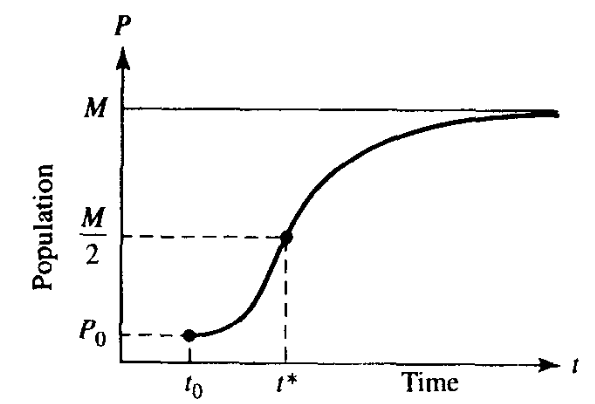
\includegraphics[width=0.5\textwidth]{logi.png}
  \end{figure}

\end{frame}

\begin{frame}{酵母增长模型}
  \begin{figure}
    \centering
    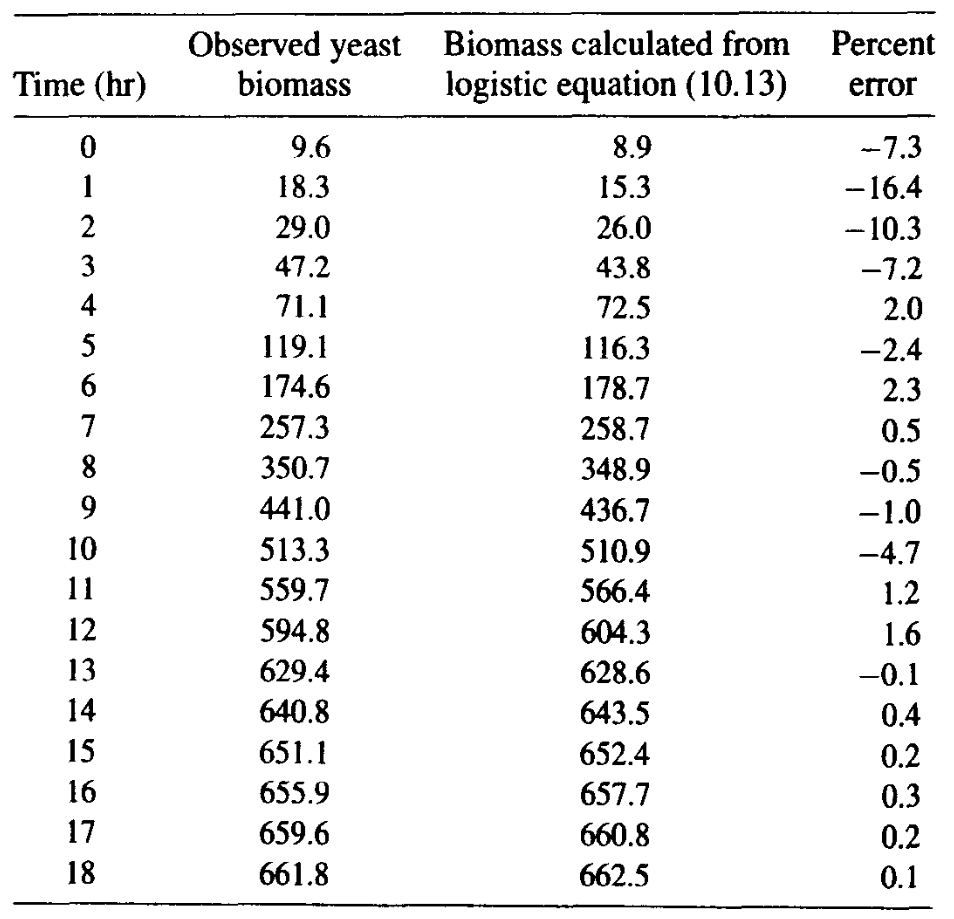
\includegraphics[width=0.6\textwidth]{yeast.png}
  \end{figure}
\end{frame}

\begin{frame}{模型拟合}
  \[
  \ln \frac{P}{M-P} = rMt + C
  \]

  \begin{figure}
    \centering
    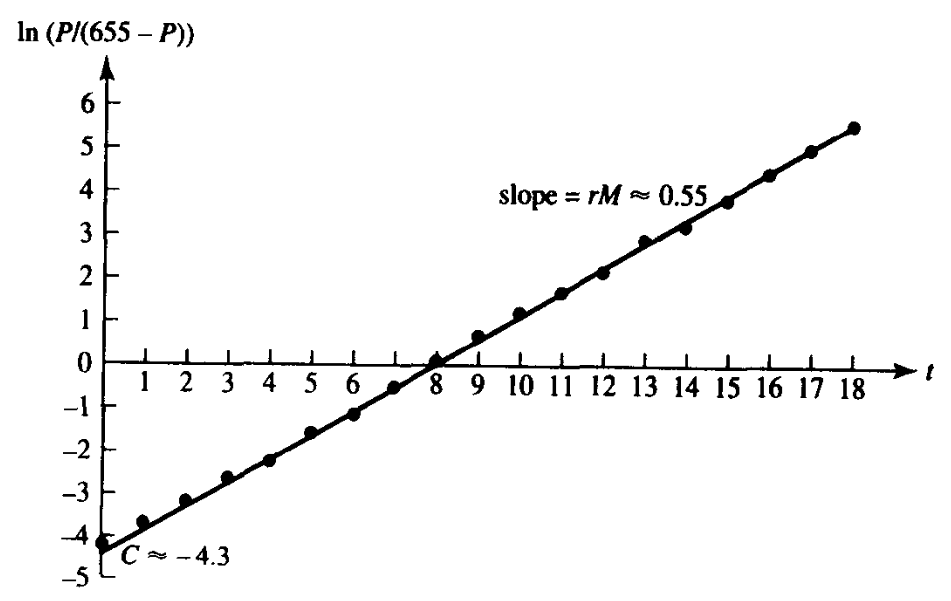
\includegraphics[width=0.6\textwidth]{yp.png}
  \end{figure}
\end{frame}

\begin{frame}{逻辑斯谛模型的另一种形式}
  设$t^*$表示$P$达到极限值$M$一半的时刻,即$P(t^*) = M/2$:

  \[
  t^* = t_0 - \frac{1}{rM} \ln \frac{P_0}{M-P_0}
  \]

  化简得:

  \[
  P(t) = \frac{M}{1 + e^{-rM(t-t^*)}}
  \]
  
\end{frame}

\begin{frame}{酵母模型拟合结果}
  \begin{figure}
    \centering
    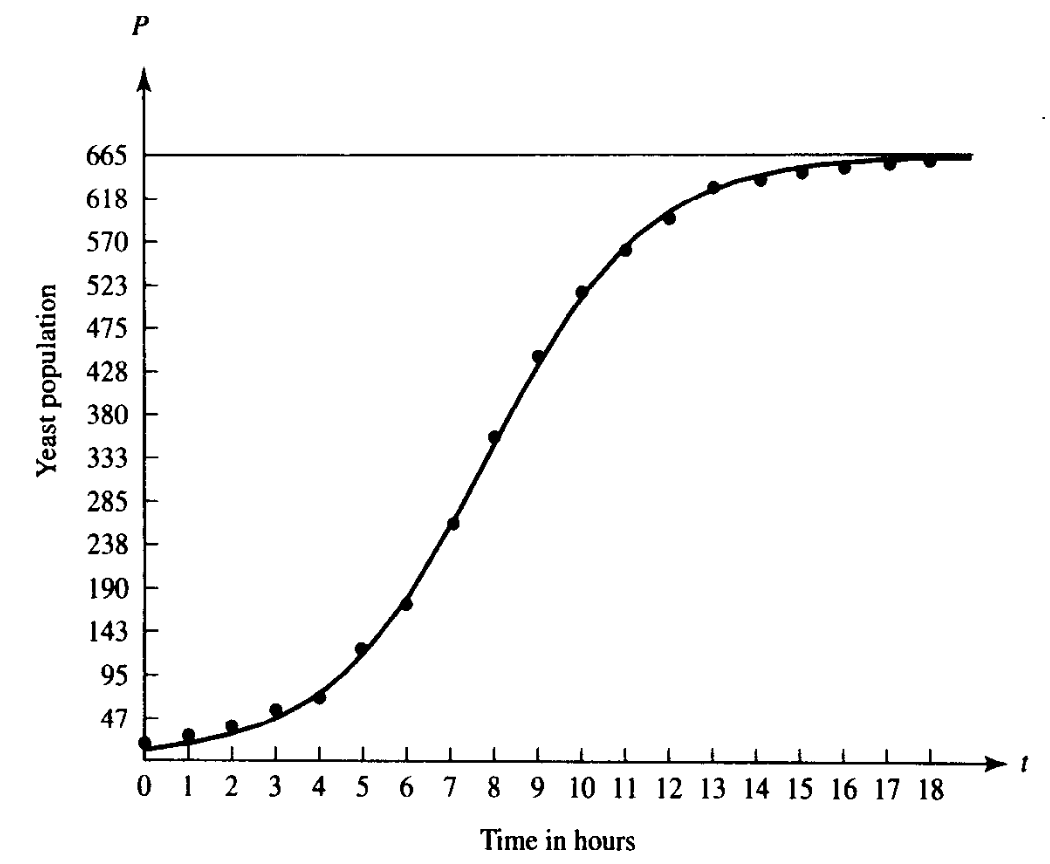
\includegraphics[width=0.6\textwidth]{yf.png}
  \end{figure}
\end{frame}

\begin{frame}{美国人口预测}
  \begin{figure}
    \centering
    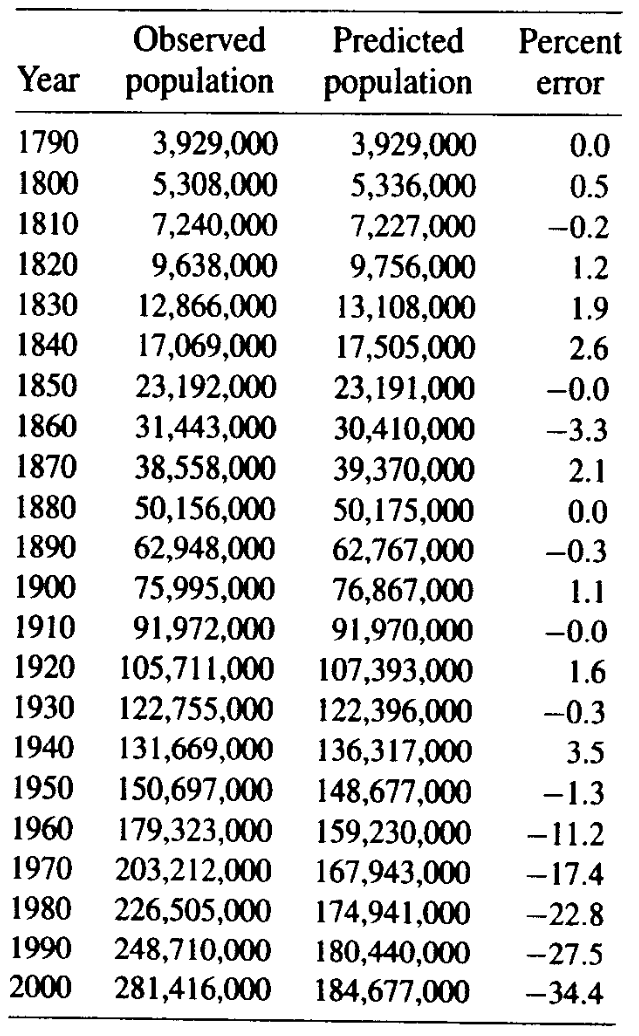
\includegraphics[width=0.4\textwidth]{ap.png}
  \end{figure}
  
\end{frame}

\begin{frame}{对药剂量开处方}
  \begin{block}{问题}
    药的剂量和用药时间应如何调节,才能保证在血液中维持安全有效的药物浓度
  \end{block}
  
  \begin{itemize}
  \item 药物浓度应介于$L$和$H$之间
  \item 如何确定用药剂量及间隔时间?
  \end{itemize}
  
  \begin{figure}
    \centering
    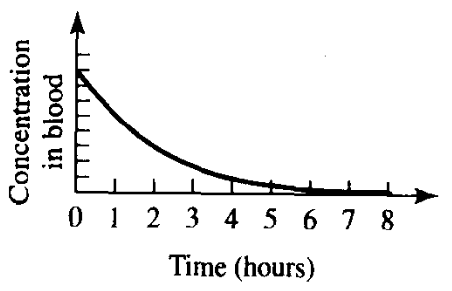
\includegraphics[height=0.25\textheight]{dd.png}
    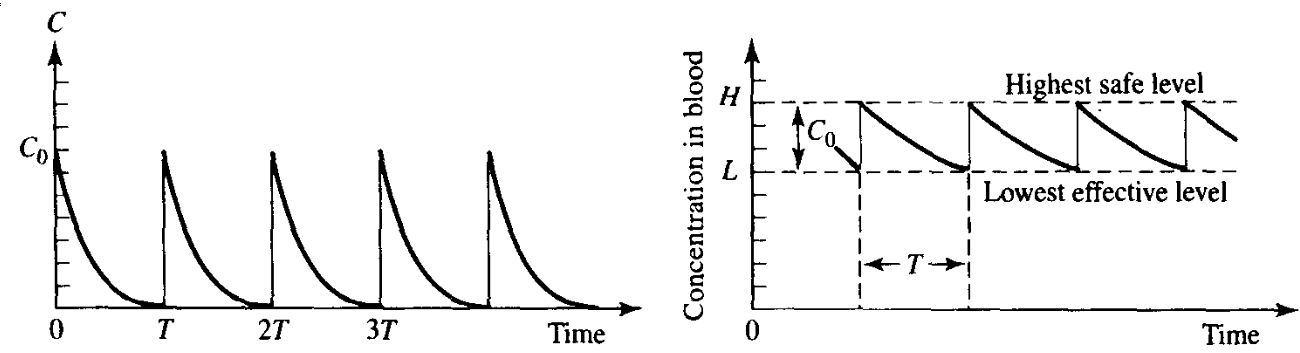
\includegraphics[height=0.25\textheight]{dr.png}
  \end{figure}
  
\end{frame}

\begin{frame}{药物减少模型}
  \begin{itemize}
  \item 实验表明,血液中药物浓度的减少与浓度成正比:$C'(t) = -kC(t)$
  \item 初始浓度$C_0 = H-L$
  \end{itemize}
  故:
  \[
  \frac{dC}{dt} = -kC, C=C_0
  \]
  \[
  C(t) = C_0e^{-kt}
  \]

  \begin{figure}
    \centering
    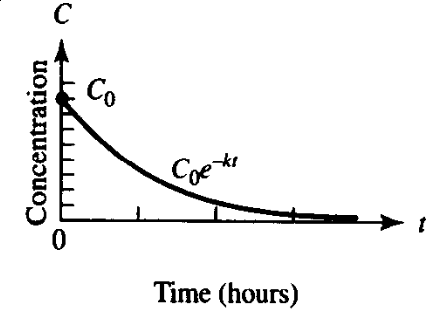
\includegraphics[width=0.4\textwidth]{dc.png}
  \end{figure}

\end{frame}

\begin{frame}{多次用药的药物积累}
  \begin{itemize}
  \item $t=0$时刻用药$C_0$
  \item $T$小时后,剩余浓度$R_1 = C_0e^{-kT}$
  \item 再服药浓度变为$C_1=C_0+C_0e^{-kT}$
  \end{itemize}

  \begin{figure}
    \centering
    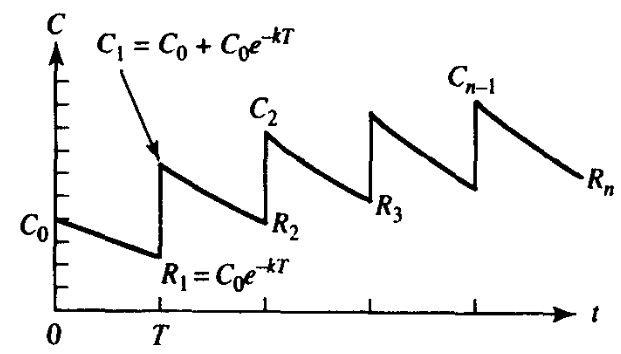
\includegraphics[width=0.5\textwidth]{ed.png}
  \end{figure}
  
\end{frame}

\begin{frame}{剩余浓度的计算}
  \begin{figure}
    \centering
    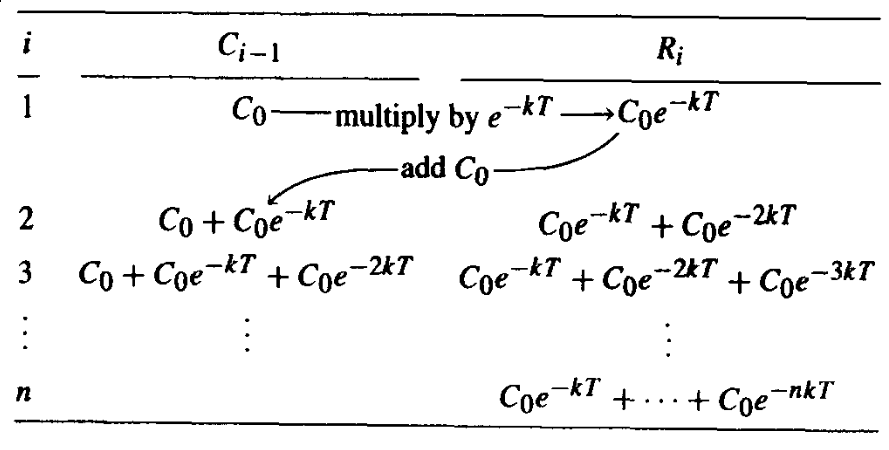
\includegraphics[width=0.5\textwidth]{rc.png}
  \end{figure}
  \[
  R_n = C_0e^{-kT}(1+r+r^2+...+r^{n-1}) = \frac{C_0e^{-kT}(1-e^{-nkT})}{1-e^{-kT}}
  \]

  \[
  R = \lim_{n \rightarrow \infty}R_n = \frac{C_0e^{-kT}}{1-e^{-kT}} = \frac{C_0}{e^{kT}-1}
  \]
  
\end{frame}

\begin{frame}{确定用药时间表}
  第$n$次间隔开始时的浓度为:

  \[
  C_{n-1} = C_0 + R_{n-1}
  \]
  
  我们希望$n$很大时,$C_{n-1}$趋近于$H$:
  
  \[
  H = \lim_{n \rightarrow \infty}C_{n-1} = \lim_{n \rightarrow \infty}(C_0+R_{n-1}) = C_0 + R
  \]
  
  同时$C_0 = H - L$,故$R=L$
  
\end{frame}

\begin{frame}{用药时间对浓度的影响}
  \[
  \frac{R}{C_0} = \frac{1}{e^{kT}-1}
  \]

  \begin{figure}
    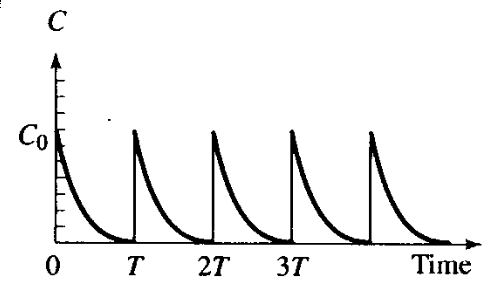
\includegraphics[width=0.4\textwidth]{lt.png}
    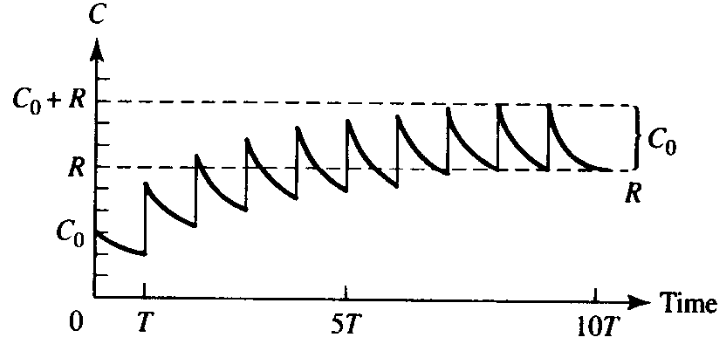
\includegraphics[width=0.5\textwidth]{st.png}
  \end{figure}
  
\end{frame}

\begin{frame}{确定用药策略}
  \[
  \left\{
  \begin{array}{l}
    C_0 = H-L\\
    R = \frac{C_0}{e^{kT}-1}\\
    R=L
  \end{array}
\right. \Rightarrow T = \frac{1}{k}\ln\frac{H}{L}
  \]

  \begin{block}{用药策略}
    第一次用药,称为承载剂量,就立即使血液中的药物浓度达到$H$,然后按照每次用药时间间隔$T=(1/k)\ln(H/L)$,将浓度提高$C_0=H-L$
  \end{block}
  
\end{frame}

\begin{frame}{微分方程解法}
  \begin{itemize}
  \item 图形解
  \item 数值近似方法
  \item 分离变量法
  \item 线性方程
  \end{itemize}
\end{frame}

\begin{frame}{Matlab解法}
  \begin{itemize}
  \item dsolve('方程1', '方程2', ..., '方程n', '初始条件', '自变量')
  \item 用字母D表示求微分, D2、D3表示求高阶微分, 如$\frac{d^2y}{dx^2}=0$表示为D2y=0
  \end{itemize}
  \begin{block}{}
    求解$\frac{du}{dt}=1+u^2$的通解
  \end{block}
  \begin{itemize}
  \item 输入命令: dsolve('Du=1+u\^\ 2', 't')
  \item 输出结果:u=tan(t-c)
  \end{itemize}
  
\end{frame}

\begin{frame}{Matlab解法}
  \begin{block}{}
  \[
  \left\{
  \begin{array}{l}
    \frac{d^2y}{dx^2} + 4\frac{dy}{dx} + 29y = 0\\
    y(0) = 0\\
    y'(0) = 15
  \end{array}
  \right.
  \]
  \end{block}

  \begin{itemize}
  \item 输入命令: dsolve('D2y + 4*Dy + 29*y=0', 'y(0)=0, Dy(0)=15', 'x')
  \item 结果:$y=3e^{-2x}sin(5x)$
  \end{itemize}
  
\end{frame}


\begin{frame}{微分方程组模型}
  \begin{block}{}
设想一个小池塘,它的环境足以维持一些野生动物的存活,我们想在池塘里放置一些供垂钓的鱼,如鳟鱼和鲈鱼。设$x(t)$表示鳟鱼在$t$时刻的数量,$y(t)$表示$t$时刻鲈鱼的数量。问这两种鱼在池塘中能否共存?如果是的话,那么这两种鱼的数量的最终解受一开始放入池塘的鱼的数量及外部干扰的敏感程度有多大?
  \end{block}

  \[
  \left\{
  \begin{array}{l}
    \frac{dx}{dt} = (a-by)x\\
    \frac{dy}{dt} = (m-nx)y\\
    x(0) = x_0\\
    y(0) = y_0
  \end{array}
  \right.
  \]
\end{frame}

\begin{frame}{微分方程组的Matlab解法}
  \begin{block}{}
  \[
  \left\{
  \begin{array}{l}
    \frac{dx}{dt}=2x-3y+3z\\
    \frac{dy}{dt}=4x-5y+3z\\
    \frac{dz}{dt}=4x-4y+2z
  \end{array}
  \right.
  \]
  \end{block}

  \begin{itemize}
  \item 输入命令: dsolve('Dx=2*x-3*y+3*z', 'Dy=4*x-5*y+3*z', 'Dz=4*x-4*y+2*z', 't')
  \item 结果:....
  \end{itemize}
  
\end{frame}

\begin{frame}{Matlab求微分方程的数值解}
  [t, x] = solver('f', ts, x0, options)

  \begin{itemize}
  \item [t] 自变量
  \item [x] 函数值
  \item [solver] ode23: 组合的二三阶的龙格-库塔-芬尔格算法,ode45:组合的四五阶的龙格-库塔-芬尔格算法,...
  \item [f] 由待解方程写成的m文件名
  \item [ts] 自变量的初值和终值
  \item [x0] 函数的初值
  \item [options] 设定误差...
  \end{itemize}

\end{frame}

\end{document}

%%% Local Variables: 
%%% TeX-master: t
%%% TeX-engine: xetex
%%% End: 
